\chapter{Implementace}

\section{Implementace API}
Implementace původně probíhala ve frameworku FastAPI \sectionref{sec:api_technologies:fast} ale po zjištění složitosti ORM při použití Python knihovny SQL Alchemy bylo doporučeno jedním z řešitelů (P. Mikula)
použít raději Javu a její Spring boot framework, za použití knihoven jako je JPA , Lombok, Jackson a jiných. Tato změna nebyla obtížná, jelikož vývoj byl teprve ve velice ranní fázi vývoje. Taktéž Spring Boot byl jeden z kandidátů.

Nyní budou popsány nejdůležitější knihovny Frameworku Spring Boot, které byly použity při implementaci API.


\subsection{Spring Boot knihovny} % TODO nějaký lepší název nebo něco

Tyto knihovny jsou základní stavební kámen jak pro samotné koncové body tak pro \gls{orm}. Na obrázku \figureref{fig:JPA} máme vizuální schéma jak magie ORM ve Spring Bootu funguje

\begin{figure}[ht!]
    \centering
    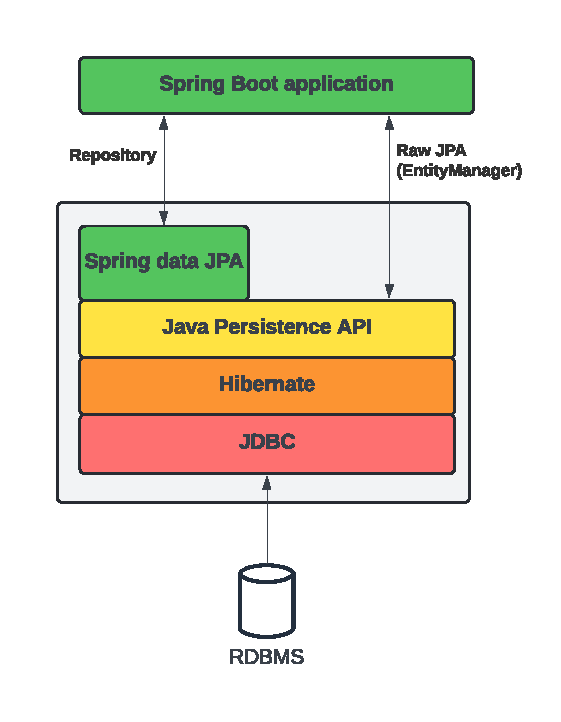
\includegraphics[width=0.8\textwidth]{figures/impl/API Implementation - JPA.pdf}
    \caption{Struktura Spring Boot Data JPA aplikace}
    \label{fig:JPA}
\end{figure}

\subsubsection*{Spring Data JPA}
Neboli Java Persistence API je jedna ze součástí Spring Data Family, která umožnuje jednoduché implementování \textbf{repozitářů} založených na JPA. Signifikantně zjednodušuje implementaci datové vrstvy aplikace. Umožňuje používat základní SQL požadavky a ORM bez námahy případně si vytvořit své vlastní požadavky. V ukázce \coderef{code:JPA_repo} je vidět implementace repositáře pro entitu \textit{Enemy}. Zde jsou již naimplementované základní metody jako \textit{save}, \textit{findAll}, a je zde navíc metoda \textit{findAllByLocationId} s vlastním SQL dotazem.

\begin{listing}[ht!]
    \inputminted[]{Java}{resources/code/impl/EnemyRepo.java}
    \caption{Ukázka JPA repositáře}
    \label{code:JPA_repo}
\end{listing}

\subsubsection*{JPA}
Spring data JPA používá několik dalších knihoven a dalo by se říci že to je jakýsi zprostředkovatel nad \textbf{JPA}. JPA je zprostředkovatel objektově relačního mapování (\gls{orm}), což usnadnuje práci s ukládáním objektů do databáze a naopak.

Základním objektem v JPA je \textit{Entita}. Ta reprezentuje objekt v databázi který je poté namapován na jednotlivé vlastnosti třídy \coderef{code:jpa_entity}.
Třídu označíme jako entitu pomocí anotace \textit{@Entity} a poté pomocí \texttt{@Table} \coderef{code:jpa_entity}[, řádek 1 a 2] můžeme upřesnit jméno tabulky, schéma databáze a jiné.Za pomoci anotace \textit{@Id} označíme primární klíč a nebo pomocí \texttt{@EmbeddedId} označíme složený primární klíč. Atributy třídy označíme pomocí \texttt{@Column} kdy ve výchozím stavu atribut může nabývat prázdné hodnoty a sloupec v databázi se jmenuje stejně jako atribut. Relace se mapují pomocí jedné z anotací \texttt{@OneToOne}, \texttt{@OneToMany}, \texttt{@ManyToOne}, \texttt{@ManyToMany} podle toho jakou relaci potřebujeme. V této implementaci probíhal nejdříve návrh databáze, takže jsme používali pouze 1:n relace abychom se vyhnuli cyklickým závislostem protože m:n spojovací tabulky již byly v databázi.

\subsubsection*{Hibernate}
Jedna z konkrétních implementací JPA je Hibernate. Udržuje si za pomocí výše zmíněných anotací nebo XML \sectionref{sec:formats:xml} schématu schéma databáze a stav objektů, tedy udržuje data perzistentní. Díky schématu databáze Hibernate ví jak se mají transformovat data z databázových tabulek do objektů a naopak. \cite[]{enwiki:1217225259}

\subsubsection*{JDBC}
Neboli Java Database Connectivity je API pro přístup k databázi.

\begin{listing}[ht!]
    \inputminted[]{Java}{resources/code/impl/EnemyDTO.java}
    \caption{Příklad entity v JPA}
    \label{code:jpa_entity}
\end{listing}


\subsection{Serializace}
\subsection{lazy load}
\section{testování}

\section{Problémy při vývoji}
\textbf{SKILL ISSUE}
\section{Další možnosti rozšíření}